\section{Auswertung}
\subsection{Zählrohr-Charakteristik}
In der Tabelle (\ref{tab:1}) sind die folgenden Messdaten aufgelistet und in
der Abbilung (\ref{abb:6}) graphisch dargestellt.
\begin{table}[H]
  \centering
  \caption{Messaufnahme zur Bestimmung des Plateaus.}
  \label{tab:1}
  \begin{tabular}{c c c c c c}
    \toprule
    $U \, /\, V$&$N$& $U \, /\, V$&$N$& $U \, /\, V$& $N$& $U \, /\, V$&$N$\\
    \midrule
\cellcolor{red}300 & \cellcolor{red}0 &410 & 13155 &530& 13336 &640& 13563\\
    310 & 12111 &420 & 13885 &540& 13225 &650& 13917\\
    320 & 12575 &430 & 12954 &550& 13318 &660& 13709\\
    330 & 12674 &450 & 13184 &560& 13376 &670& 13721\\
    340 & 12504 &460 & 13193 &570& 13200 &680& 13918\\
    350 & 12753 &470 & 13011 &580& 13514 &690& 13663\\
    360 & 12838 &480 & 13205 &590& 13438 &700& 14302\\
    370 & 12961 &490 & 13022 &600& 13363 &-& -\\
    380 & 12936 &500 & 13303 &610& 13288 &-& -\\
    390 & 12794 &510 & 13076 &620& 13446 &-& -\\
    400 & 13076 &520 & 13363 &630& 13495 &-& -\\
    \bottomrule
  \end{tabular}
\end{table}
\begin{figure}[H]
  \centering
  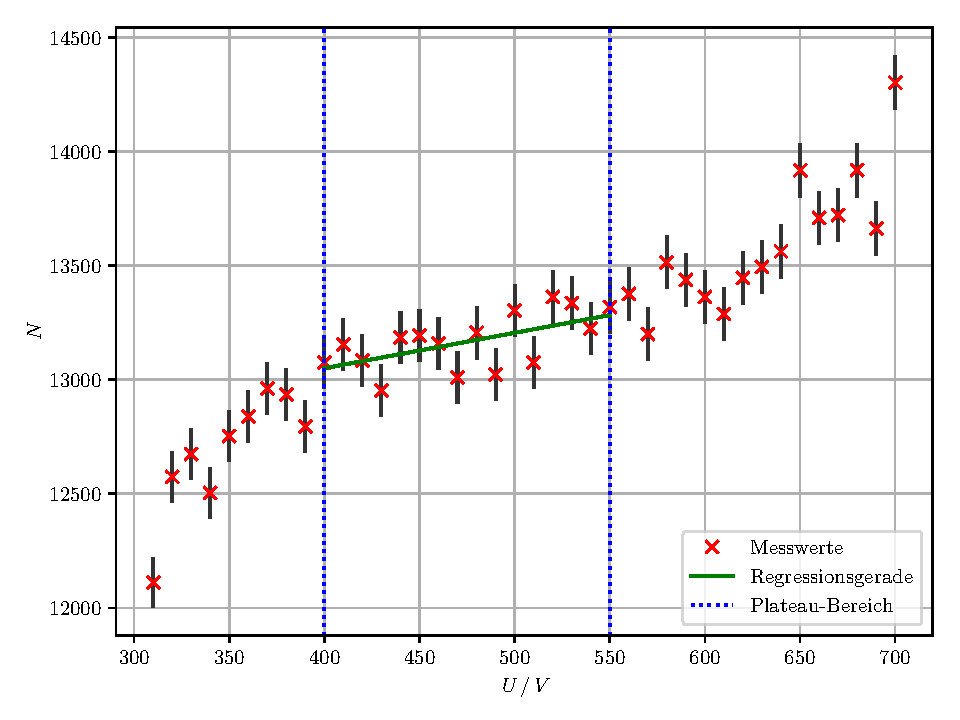
\includegraphics{plot1.pdf}
  \caption{Darstellung der Messdaten mit Fehlerbalken sowie die Einnteilung des Plateaus.}
  \label{abb:6}
\end{figure}
Es ist zu beachten, dass der erste Messwert (rötlich hinterlegt) nicht in der Auswertung berücksichtig wird,
da sie physikalisch nicht sinnvoll ist.
Die Länge des Plateaus beginnt bei $400 V$ und endet bei $550 V$. Für diesen Kurvenabschnitt wird eine lineare Auschgleichsrechnung
\begin{align}
  y & = m \cdot x + b \label{eq:9}\\
  m & = \frac {\bar{xy} - \bar{x} \cdot \bar{y}} {\bar{x^2} -\bar{x}^2}&  \label{eq:10}\\
  b & = \frac {\bar{y} \cdot \bar{x}^2 - \bar{xy} \cdot \bar{x}} {\bar{x^2}-\bar{x}^2}& \label{eq:11}
\end{align}
durchgeführt.
Somit ergibt sich für die Parameter der Geraden:
\begin{itemize}
  \item m = 1.55 \pm 0,55 SI{\per\volt}
  \item b = 12429,16 \pm 264,59
\end{itemize}

Anschließend wird die Plateau-Steigerung in $\%$ pro $100 V$ mit
\begin{equation}
  s = \frac{f(500)}{f(400)} \cdot 100 - 100 \%
\end{equation}
bestimmt.
Die Steigerung beträgt $s = 1.2 \pm 0.4 \SI{\%\per\volt}$ liegt.
 
